%!Tex root=ZF_bmicha_TRM.tex
\subsection{Rigid Body Transformation}
    A mapping $g$ is a rigid body transformation if:
    \begin{itemize}
        \item \textbf{length} (distances between pts.) is preserved
            $$
                \lVert g(q) - g (p) \rVert = \lVert q - p \rVert
            $$
        \item \textbf{crossproduct} (orientation) is preserved:
            $$
                g(v\times w) = g(v) \times g(w)
            $$
    \end{itemize}
\subsection{Mathematical Remarks}
    \subsubsection{Skew - Symmetric Matrix \texorpdfstring{\hfill $\widehat{a}$}{}}
        \vspace{-1em}
        $$
            a \times b = \widehat{a} b = 
            \begin{bmatrix}
                0   & -a_3 &  a_2\\
                a_3 &    0 & -a_1\\
                -a_2&  a_1 &    0
            \end{bmatrix}
            b
            =
            \begin{bmatrix}
                a_2 b_3 - a_3 b_2\\
                a_3 b_1 - a_1 b_3\\
                a_1 b_2 - a_2 b_1
            \end{bmatrix}
        $$
    \subsubsection{Matrix Exponential}
        \vspace{-0.5em}
        \begin{align*}
            e^{\widehat{\omega} \theta} &= \mathbb{I} + \widehat{\omega} \theta + \frac{1}{2!} (\widehat{\omega} \theta)^2 + \frac{1}{3!} (\widehat{\omega} \theta)^3 + \dots\\[0.5em]
                                        &\overset{*}{=} \mathbb{I} + \widehat{\omega} \sin\theta + \widehat{\omega}^2 (1 -\cos\theta)
        \end{align*}
        $(*)$ Rodrigues' Formula
\subsection{Screw Parameters \& Twist}
        All parameters respresented in \textbf{reference frame}.
    \begin{description}
        \item[Pitch $h$]: Ratio of translational and rotational motion
        \item[Axis $l$]: Axis of rotation / direction of translation
        \item[Magnitude $M$]: Amount of rotation/ translation  
        % \item[Twist $\widehat{\xi}$]
        % \item[Twist Coordinates $\xi$] 
    \end{description}

    \subsubsubsection{General Case}
        \begin{align*}
            h = \frac{\omega^T v}{\lVert \omega^2 \rVert} && l = \frac{\omega \times v}{\lVert \omega^2 \rVert} + \lambda \omega && M = \lVert \omega \rVert
        \end{align*}
        \begin{align*}
            \widehat{\xi} &= 
                \begin{bmatrix}
                    &\widehat{\omega} & & - \omega \times q + h \omega\\
                    0 & 0 & 0 & 0 \\
                \end{bmatrix}
            &\in \mathbb{R}^{4 \times 4}\\
            \xi &= 
                \begin{bmatrix}
                    - \omega \times q + h \omega\\
                    \omega
                \end{bmatrix}
            &\in \mathbb{R}^{6 \times 1}
        \end{align*}
    \subsubsubsection{Rotation}
        \begin{align*}
            h = 0 && l = q + \lambda \omega && M = \theta
        \end{align*}
        \begin{align*}
            \widehat{\xi} &= 
                \begin{bmatrix}
                    &\widehat{\omega} & & - \omega \times q\\
                    0 & 0 & 0 & 0 \\
                \end{bmatrix}
            \\
            \xi &= 
                \begin{bmatrix}
                    - \omega \times q\\
                    \omega
                \end{bmatrix}
        \end{align*}
    \subsubsubsection{Translation}
        \begin{align*}
            h = \infty && l = \lambda v && M = \theta
        \end{align*}
        \begin{align*}
            \widehat{\xi} &= 
                \begin{bmatrix}
                    0 & v\\
                    0 & 0 \\
                \end{bmatrix} \in \mathbb{R}^{4 \times 4}
            \\
            \xi &= 
                \begin{bmatrix}
                   v\\
                   0    
                \end{bmatrix} \in \mathbb{R}^{6 \times 1}
        \end{align*}
    \subsection{Matrix Exponentials}
        \vspace{-1em}
        $$\boxed{%
            g_{st}(\theta_1,\dots ,\theta_n) = e^{\widehat{\xi}_1 \theta_1} \cdots e^{\widehat{\xi}_n \theta_n} \cdot g_{st}(0) = H_n^0
        }$$
        $g_{st}(0)$: IC of $n^{th}$ frame w.r.t. $0^{th}$ frame.
    \subsubsection{Homogeneous Transformation}
    The twist matrix exponential yields a Homogeneous Transformation. For $\lVert \omega \rVert = \lVert v \rVert = 1$
    $$
        e^{\widehat{\xi} \theta} =
        \begin{bmatrix}
            e^{\widehat{\omega} \theta} & \left( \mathbb{I} - e^{\widehat{\omega} \theta} \right) ( \omega \times v) + h \theta \omega\\
            0 & 1
        \end{bmatrix} \in \mathbb{R}^{4 \times 4}
    $$
    \vskip0.5em
    \begin{minipage}{0.49\linewidth}
        \begin{center}
            \textbf{Revolute}
        \end{center}
        $$
            \begin{bmatrix}
                e^{\widehat{\omega} \theta} & \left( \mathbb{I} - e^{\widehat{\omega} \theta} \right) ( \omega \times v)\\
                0 & 1
            \end{bmatrix}
        $$
    \end{minipage}
    \begin{minipage}{0.49\linewidth}
        \begin{center}
            \textbf{Prismatic}
        \end{center}
        $$
            \begin{bmatrix}
                \mathbb{I} & \theta v\\
                0 & 1
            \end{bmatrix}
        $$
    \end{minipage}
    \subsubsection{Initial Coniditions}
        \vspace{-1em}
        $$\boxed{%
            g_{ab}(\theta) = e^{\widehat{\xi} \theta} \cdot g_{ab}(0)
        }$$
        \textbf{$g_{ab}(0)$} describes transformation from base to toolframe.
        $$
            g_{ab}(0) = \begin{bmatrix}
                R(0) & q\\
                0 & 1
            \end{bmatrix}
        $$  
\subsection{Matlab - Kinematics Toolbox}
    \begin{center}
        \resizebox{0.78\linewidth}{!}{
        % \resizebox{0.94\linewidth}{!}{
                \includegraphics[
                    page = {11},
                    % trim = {2.5cm, 1.6cm, 2.9cm, 2.5cm}, % with blue frame
                    trim = {2.9cm, 2cm, 3.4cm, 2.9cm}, %left bottom right top
                    clip
                ]{Screw_Theory/02_2020-10-06_ScrewTheory.pdf}
            } 
    \end{center}
    